% Dokumenttyp
\documentclass[a4paper,11pt,twoside,german]{article}

% Befehle für Seitenränder
\newcommand{\largeborder}{3cm}
\newcommand{\smallborder}{2cm}
\newcommand{\topborder}{1cm}
\newcommand{\bottomborder}{1cm}

\usepackage[
    left=\largeborder,
    right=\largeborder,
    top=\topborder,
    bottom=\bottomborder,
    includeheadfoot,
    ]{geometry}
    
% \textwidth 16cm
% \textheight 24cm
%  \topmargin -15mm
% \setlength{\oddsidemargin}{-5mm}
% \setlength{\evensidemargin}{5mm}


%%%%%%%%%%%%%%%%%%%%%%%%%%
%%% Benötigte Packages %%%
%%%%%%%%%%%%%%%%%%%%%%%%%%

%%% Sprache %%%
\usepackage[ngerman]{babel}    	% damit man deutsche Dinge tun kann
\usepackage{ziffer} % Deutsche Zahlen

\usepackage[utf8]{inputenc}   % damit Umlaute funktionieren
\usepackage[autostyle=true,german=quotes]{csquotes} % Anführungszeichen richtig
\usepackage{blindtext} % damit man sinnlosen Text produzieren kann

%%% Grafiken %%%
\usepackage{graphicx}    % damit man Bilder einbinden kann
% \usepackage{float}    	% damit Floats da sind, wo sie hingehören
\usepackage{floatrow}   % bessere float Organisation
\usepackage[font=footnotesize,labelfont=bf,skip=0pt]{caption} %Captions anpassen
\addtolength{\intextsep}{2mm} % mehr Platz um figures und tables
\usepackage{subcaption}
\usepackage{pbox}


\usepackage{amsmath}  % damit abgefahrene mathematische Dinge in equations gehen
\usepackage{enumitem} % Damit Aufzählungen hübscher sind
\usepackage{ifthen}   % Damit man if-else-Strukturen machen kann

\setlength{\parindent}{0pt} % Keine Absatzeinrückung
\usepackage{setspace} % Zeilenabstände machen können
\linespread{1.1} % Zeilenabstand definieren
% Standardmäßig \absatz zur Trennung von Absätzen verwendet und hier anpassen
\newcommand{\absatz}{\smallbreak} 
%\renewcommand{\familydefault}{\sfdefault} % Serifenlose Schrift

%%% Links und Verweise %%%
\usepackage[breaklinks]{hyperref} % Damit Links funktionieren
\hypersetup{colorlinks=false,pdfborder={0 0 0}} % entferne hässliche Link-Kästen


%%% Bibliographie %%%
\usepackage[authoryear,round]{natbib} % Der Stil der LiteraturVERWEISE im Text
\bibliographystyle{dcu-german-spec} % Der Stil des LiteraturVERZEICHNISSES
%\bibliographystyle{dcu} % Der Stil des LiteraturVERZEICHNISSES


% Makro für Bibliographie
\newcommand{\literaturverzeichnis}[1]{
    \renewcommand{\harvardand}{und} % ein UND statt AND bei mehreren Autoren
    \bibliography{#1}
    }

% Literaturverzeichnis im Inhaltsverzeichnis, aber NICHT nummeriert
\usepackage[nottoc,notlot,notlof]{tocbibind} 
% Literaturverzeichnis nummeriert und im Inhaltsverzeichnis
% \usepackage[nottoc,numbib]{tocbibind}


% Commands to place things on a left or right side
% Put this before something you want to place either right 
% (onto the NEXT EVEN page) or left (onto the NEXT ODD page)
\newcommand{\emptypage}{\newpage\leavevmode\thispagestyle{empty}\newpage}
\newcommand{\fillwithemptypagestillevenside}{\ifthenelse{\isodd{\thepage}}
    {\emptypage}{}}
\newcommand{\fillwithemptypagestilloddside}{\ifthenelse{\isodd{\thepage}}{}
    {\emptypage}}

\newcommand{\breaktoevenside}{\ifthenelse{\isodd{\thepage}}{\newpage}{}}
\newcommand{\breaktooddside}{\ifthenelse{\isodd{\thepage}}{}{\newpage}}

% Metadaten
\usepackage{titling}
\title{LEX extended abstract}
\author{
    Büchau, Yann Georg \\
    \small{\texttt{64\,36\,211}}
    \and
    Finn, Tobias Sebastian \\
    \small{\texttt{00\,00\,000}}
    \and 
    Schaper, Maximilian \\
    \small{\texttt{00\,00\,000}}
    }
%%%%%%%%%%%%%%%%%%%%%%%%%%%%%%%%%%%%%%%%%%
\begin{document}
\raggedbottom


%%%%%%%%%%%%%%%%%%
%%% Titelseite %%%
%%%%%%%%%%%%%%%%%%

\hypersetup{pageanchor=false}
\makeatletter
\begin{titlepage}

%\newgeometry{
%    left=\smallborder,
%    right=\smallborder,
%    top=\topborder,
%    bottom=\bottomborder,
%    includeheadfoot,
%    }


\vspace*{\fill}
\begin{center}
\Large{\textbf{Lehrexkursion Fehmarn}}\\
\large{29.08.2016 - 09.09.2016}\\
\vspace{5mm}
\Large{\textbf{Arbeitsgruppe\\Wolkenkamera Stereo}}\\
\vspace{1cm}

% authors
\begin{large}
\begin{tabular}{ccc}
Büchau, Yann Georg & Finn, Tobias Sebastian & Schaper, Maximilian \\
\small{\texttt{64\,36\,211}} & 
\small{\texttt{00\,00\,000}} &
\small{\texttt{00\,00\,000}}
\end{tabular}
\end{large}

\vspace{1cm}
\large{Meteorologisches Institut}\\
\large{Universität Hamburg}\\
\vspace{1cm}
\large{{\today}}
\end{center}
\vspace*{\fill}

\clearpage
% \restoregeometry


\end{titlepage}
\makeatother
\hypersetup{pageanchor=true}

\newpage

%%%%%%%%%%%%%%%%%%%%%%%%%%
%%% Inhaltsverzeichnis %%%
%%%%%%%%%%%%%%%%%%%%%%%%%%
\clearpage
\setcounter{page}{1} % Page counting begins here!

\tableofcontents % Inhaltsverzeichnis
\vspace*{\fill}

%%%%%%%%%%%%%%%%%%%%%%%%%%%%%
%%% Abbildungsverzeichnis %%%
%%%%%%%%%%%%%%%%%%%%%%%%%%%%%
\listoftables % Abbildungsverzeichnis

\listoffigures % Abbildungsverzeichnis

\newpage


%%%%%%%%%%%%%%%%%%
%%% Motivation %%%
%%%%%%%%%%%%%%%%%%
\section{Motivation}

Ceilometer sind teuer, Kameras sind billig und vielseitig (Bedeckungsgrad,
Höhenwind, Wettergeschehen, etc...).  Es lohnt sich daher die Untersuchung,
inwiefern die Wolkenhöhe auch mit Kameras bestimmt werden kann.

%\newpage

%%%%%%%%%%%%%%
%%% Geräte %%%
%%%%%%%%%%%%%%
\section{Geräte}

Die verwendeten zwei Kameras (Abbildung \ref{FIGKameras}) werden im Folgenden
\enquote{Acker} und \enquote{Feld} genannt. Es handelt sich um
Überwachungskameras VIVOTEK FE8174V mit einem Blickfeld von nahezu $180^\circ$
und einer Bildauflösung von $1920\,\mathrm{px} \cdot 1920
\,\mathrm{px}$.
\absatz

\begin{figure}[!h]
\begin{center}
\scriptsize
\begin{minipage}{0.45\textwidth}
    \bgroup
    \def\arraystretch{0.2}
    \begin{tabular}{cc}
    Kamera \enquote{\textbf{Acker}} & Kamera \enquote{\textbf{Zaun}} \\
    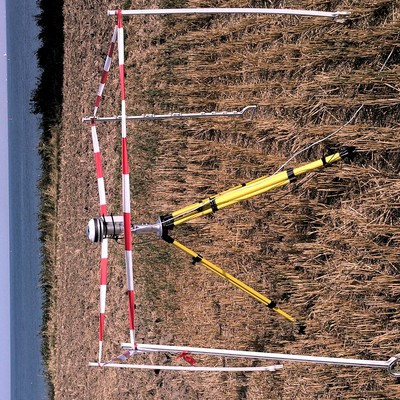
\includegraphics[width=0.45\textwidth, angle=-90]{media/cam4.jpg} &
    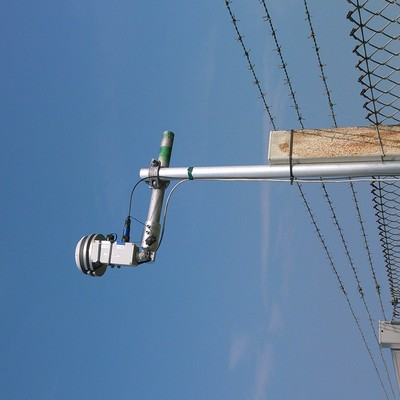
\includegraphics[width=0.45\textwidth, angle=-90]{media/cam3.jpg} \\
    \end{tabular}
    \egroup
\end{minipage}
\begin{minipage}{0.45\textwidth}
    \bgroup
    \def\arraystretch{2}
    \scriptsize
    \begin{tabular}{ccc}
    & 
    \pbox{\textwidth}{Kamera\\ \enquote{\textbf{Acker}}} &
    \pbox{\textwidth}{Kamera\\ \enquote{\textbf{Zaun}}} \\
    \hline
    \pbox{\textwidth}{\textbf{GPS Position}} & 
    \pbox{\textwidth}{$54,4959^\circ\,\mathrm{N}$ \\
    $11,2377^\circ\,\mathrm{O}$} &
    \pbox{\textwidth}{$54,4947^\circ\,\mathrm{N}$ \\ $11,2408^\circ\,\mathrm{O}$} \\
    \hline
    \pbox{\textwidth}{\textbf{Höhe über N.N.}} & 
    $0\,\mathrm{m}$ &
    $9\,\mathrm{m}$ \\
    \hline
    \end{tabular}
    \egroup
\end{minipage}
\vspace{-0.5cm}
\caption[verwendete Kameras]{Kameras \enquote{Acker} und \enquote{Zaun} mit
Koordinaten. Kamera \enquote{Zaun} befand sich auf dem Militärgelände
Marienleuchte, Kamera \enquote{Acker} etwa $241\,\mathrm{m}$ entfernt auf einem
Feld.}
\label{FIGKameras}
\end{center}
\end{figure}


%\newpage % Neue Seite 

%%%%%%%%%%%%%%%%%%%
%%% Kalibration %%%
%%%%%%%%%%%%%%%%%%%
\section{Kalibration}

Grundlegend für die im Folgenden angewendete Triangulationsmethode ist die
Kenntnis des Azimuth- und Elevationswinkels in jedem Bildpunkt. Dazu ist eine
Kalibration der verwendeten Kameras erforderlich, mit der sowohl die radiale
Projektion der Kameralinse als auch die Drehungseffekte durch ungenaues
Aufstellen der Kamera quantifiziert werden können. Für eine derartige
Kalibration sind Raumpunkte nötig, deren Positionen sowohl auf dem Bild als auch
in der Realität bekannt sind. Es bietet sich hierfür die Sonne an, deren realer
Azimuth- und Elevationswinkel zu jedem Zeitpunkt berechenbar sind
\citep{pysolar}.
\absatz 
Bedeckt man eine Kamera an einem nahezu wolkenlosen
Tag mit Goldfolie und verringert die Belichtungszeit \citep{ingo}, erscheint die
Sonne als einziger heller Fleck auf dem ansonsten dunklen Bild (Abbildung
\ref{FIGFolie}).  Das ermöglicht die programmatische Bestimmung der
Sonnenposition auf dem Bild mittels Weichzeichnung, Erosion kleiner Elemente und
Mittelpunktsbestimmung des hellsten Bildbereichs.
\absatz
Zur Bestimmung von Azimuth- und Elevationswinkel in jedem Bildpunkt wird eine
Projektion benötigt, mit der sich Bildkoordinaten $\left[Zeile \,\,
Spalte\right]$ in das reale, dreidimensionale Koordinatensystem
$\left[X\,\,Y\,\,Z\right]$ umrechnen lassen.  Eine solche Projektion ist in
Abbildung~\ref{FIGProjektion} gezeigt. Dabei wird zunächst anhand des Bildradius
$R_\mathrm{h}$, also des Abstandes des betrachteten Bildpunktes zur Bildmitte in
Bildpunktbreiten, der Lotwinkel $\phi$ zur optischen Achse angenährt. Er lässt
sich umrechnen in die Elevation $\epsilon = \frac{\pi}{2} - \phi$. Dem liegt die
Annahme zugrunde, dass es sich um eine radiale Verzerrung handelt, die
rotationssymmetrisch zur in der Bildmitte liegenden optischen Achse der Linse
ist.  Dieser Schritt quantifiziert also den Verzerrungseffekt der Linse. Hier
wird nach \cite{ingo} ein Polynom vierten Grades als Zusammenhang angenommen und
invertiert:

\begin{equation}
\label{GLRadial}
R_\mathrm{h} = p_4 \phi ^ 4 + p_3 \phi ^ 3 + p_2 \phi ^ 2 + p_1 \phi
\end{equation}

Durch die nun bekannte Elevation wird der Vektor des betrachteten Bildpunktes
dreidimensional. Zur Nordung wird der Vektor anschließend um den Winkel $\Phi_Z$
um die $Z$-Achse gedreht. Eine weitere Drehung um den Winkel $\Phi_X$ um die
$X$-Achse und um den Winkel $\theta_Z$ um die dann mitbewegte $Z$-Achse
korrigieren den Vektor um Fehler, die bei der Ze\-nit\-aus\-rich\-tung der
Kamera gemacht wurden. Diese drei Winkel $\Phi_Z$, $\Phi_X$ und $\theta_Z$
werden auch als Euler-Winkel bezeichnet.
\absatz
Die Kalibration kann somit als Optimierungsproblem betrachtet werden. Dazu
werden alle auf den Kamerabildern gefundenen Sonnenpositionen auf eine
Einheitssphäre im realen Koordinatensystem projiziert. Der mittlere quadratische
Abstand zu den tatsächlichen Sonnenpositionen auf der Einheitssphäre ist die zu
optimierende Kostenfunktion in Ab\-häng\-ig\-keit der Projetionsparameter $p_1$,
$p_2$, $p_3$, $p_4$, $\Phi_Z$, $\Phi_X$ und $\theta_Z$.
\absatz
Dieser Kalibrationsansatz lässt sich theoretisch sowohl für jede Aufstellung
einer Kamera, als auch für jede Art von Kamera anwenden. Allerdings wird es bei
anderen Kameras eventuell nötig sein, die radiale Projektionsfunktion in
Gleichung \ref{GLRadial} anzupassen, wenn sich die Art der Linse stark von der
hier verbauten unterscheidet.
\absatz
Die radiale Projektionsfunktion ist gerätespezifisch. Somit sind die Parameter 
$p_1$, $p_2$, $p_3$ und $p_4$ unabhängig von der Aufstellung. Daher bietet es
sich an, die Projektionsfunktion separat zu bestimmen und für jede
Kameraaufstellung zu übernehmen. Für eine optimale Genauigkeit sind
möglichst viele Sonnenpositionen auch in der Bildmitte erforderlich, was bei
einer Ausrichtung in den Zenith in den mittleren Breiten nicht erfüllt ist.
Richtet man die Kamera aber in Richtung der Mittagssonne aus, ist diese
Vorraussetzung erfüllt, wie in Abbildung \ref{FIGFolie}(b) zu sehen ist.
Mit dieser Aufstellung ergeben sich für die Kamera \enquote{Zaun} 
die folgenden Radialprojektionsparameter:

\begin{equation}
p_4 = -20,933 \;\;\;\;
p_3 = 0,536   \;\;\;\;
p_2 = 25,295  \;\;\;\;
p_1 = 658,265 \;\;\;\;
\end{equation}

Da die beiden hier verwendeten Kameras baugleich sind, wird für Kamera
\enquote{Acker} dieselbe Projektionsfunktion angenommen.  Mit dieser
Projektionsfunktion (Abbildung \ref{FIGProjektioncalib}) können jetzt die in den
Zenith gerichteten Kameraaufstellungen kalibriert werden wie etwa in Abbildung
\ref{FIGFolie}(a) zu sehen. Aus den daraus gewonnenen Parametern lassen sich wie
gewünscht für jeden Bildpunkt ein Azimuth- und Elevationswinkel bestimmen. 
\absatz 
Eine Koordinatentransformation kann dann dazu verwendet werden, die
Bilder zu entzerren. Dazu wird ein Gitter aus equidistanten $X$ und $Y$
Koordinaten erstellt und eine virtuelle, konstante Höhe $Z$ angenommen. Diese
virtuelle Höhe $Z$ hat keine Verbindung zu der Wolkenhöhe, sondern dient nur der
Darstellung einer Ebene. Aus diesen Koordinaten werden Azimuth und Elevation
berechnet und dann darauf das Kamerabild auf Basis seiner kalibrierten Azimuth-
und Elevationswinkel intepoliert.

\begin{figure}[!h]
\begin{center}
\begin{floatrow}
\ffigbox{
    \caption[Sonnenbahn auf mit Goldfolie bedeckter Kamera]{
    Zusammenstellung ausgewählter Aufnahmen der mit Goldfolie bedeckten Kamera
    \enquote{Zaun} bei einer groben Ausrichtung der optischen Achse (Bildmitte)
    (a) in den Zenith und (b) in die Mittagssonne.
    }
    \label{FIGFolie}
}{
    \begin{tabular}{cc}
        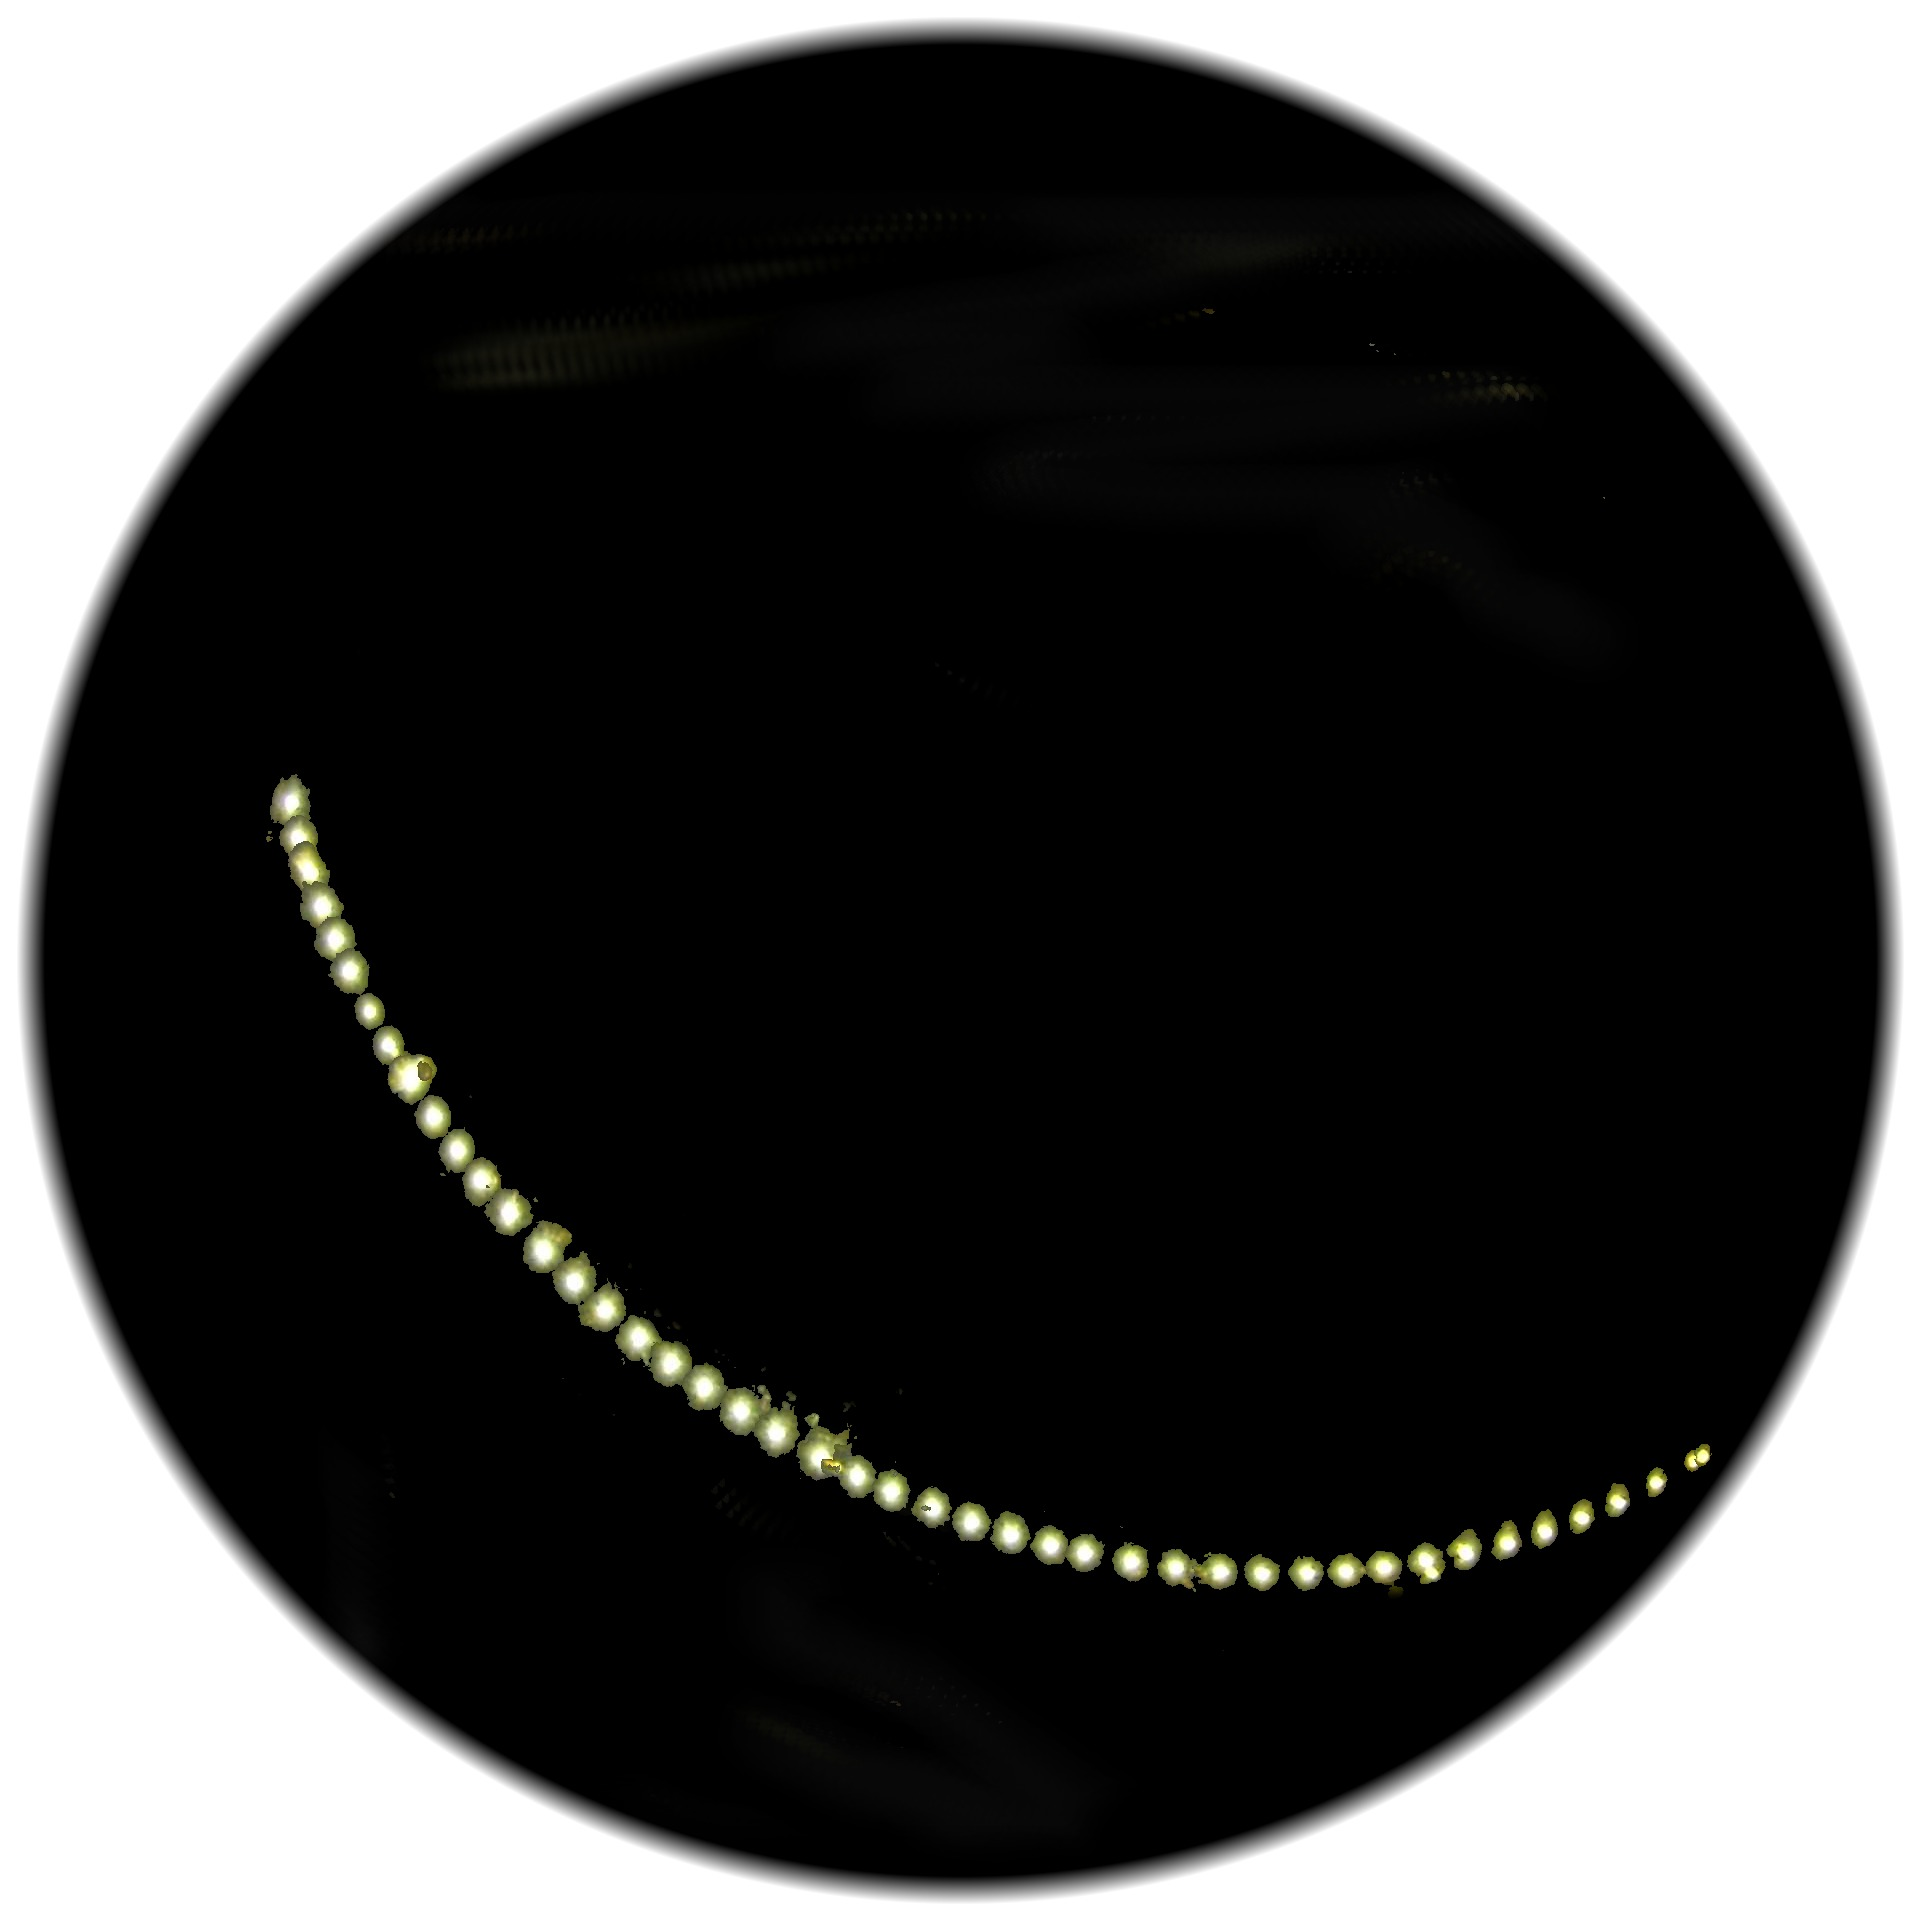
\includegraphics[width=0.22\textwidth]{media/cam3_straight_gold.jpg} &
        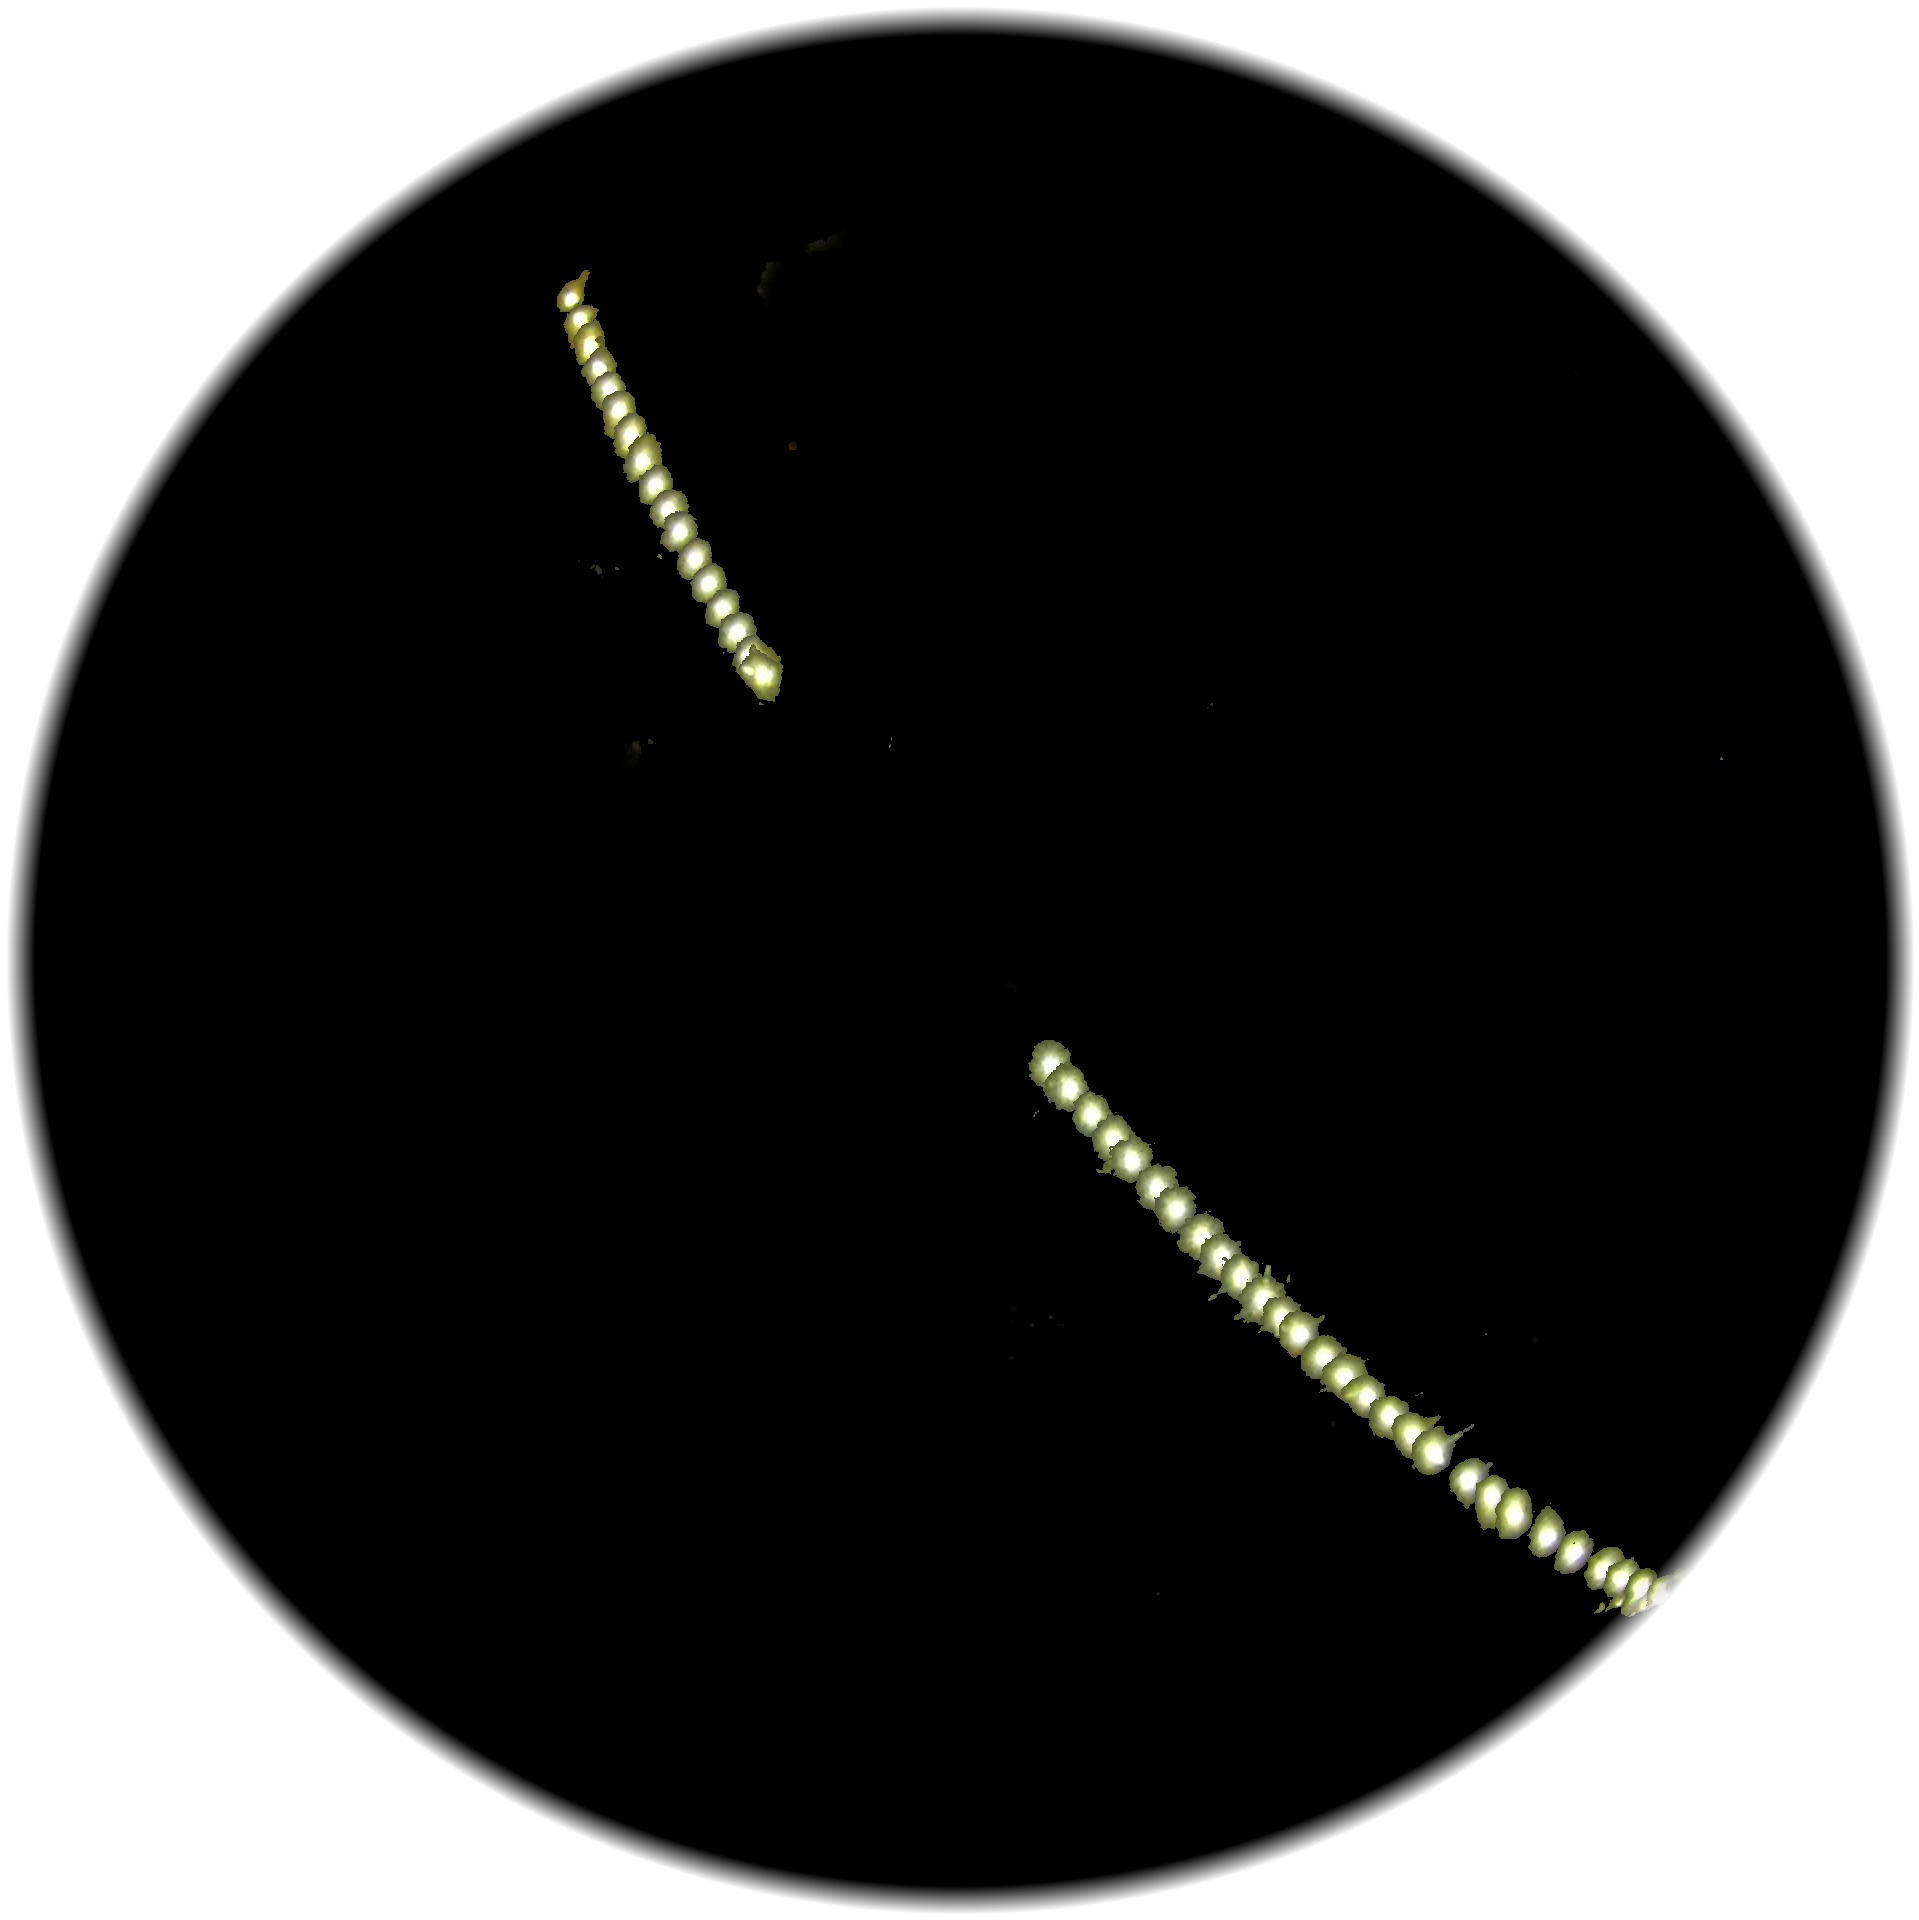
\includegraphics[width=0.22\textwidth]{media/cam3_proj_gold.jpg} \\
        (a) & (b) \\
    \end{tabular}
    }
    
\ffigbox{
    \caption[Projektion von Bildkoordinaten zu realen Koordinaten]{Projektion
    von Bildkoordinaten zu realen Koordinaten: (1) Sonne auf dem Bild (2)
    Elevation wird aus Radialprojektion angenährt (3)\,-\,(5) Drehung im Raum
    durch Euler-Winkel.  Die Punkte\ (2)\,-\,(5) befinden sich auf der
    Einheitsphäre.}
    \label{FIGProjektion}
}{
    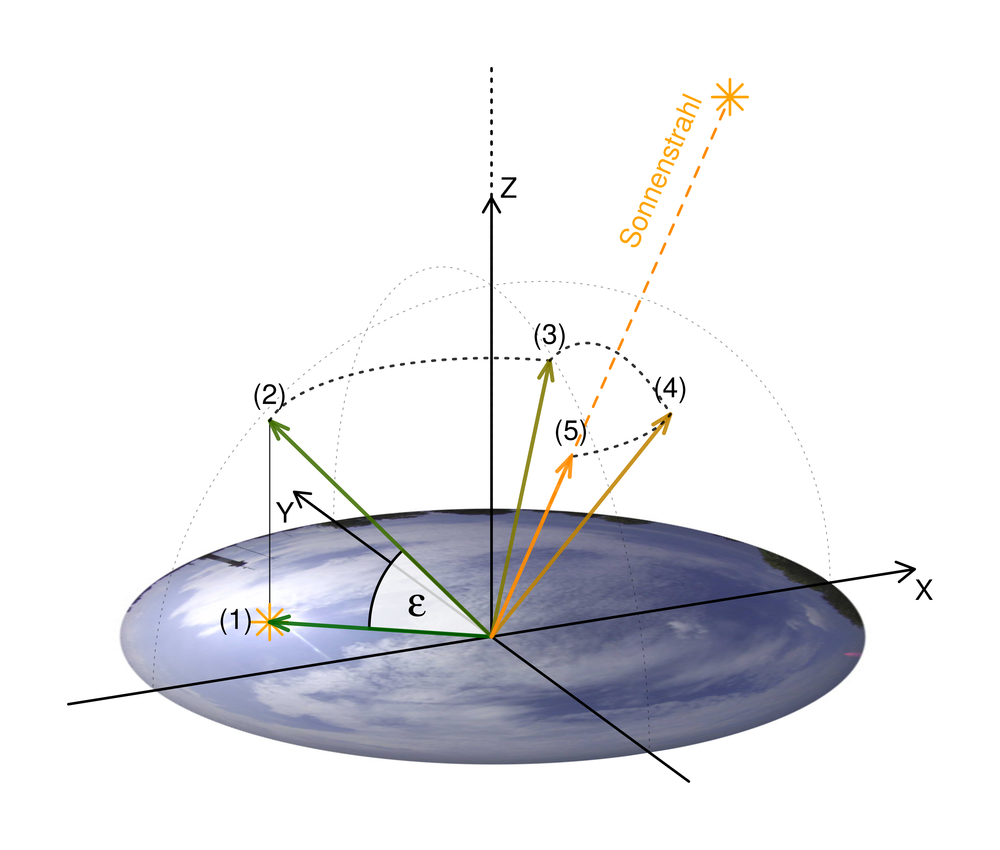
\includegraphics[width=0.49\textwidth]{media/calibration-chart.png}
}
\end{floatrow}
\end{center}
\end{figure}

\begin{figure}[!h]
\begin{center}
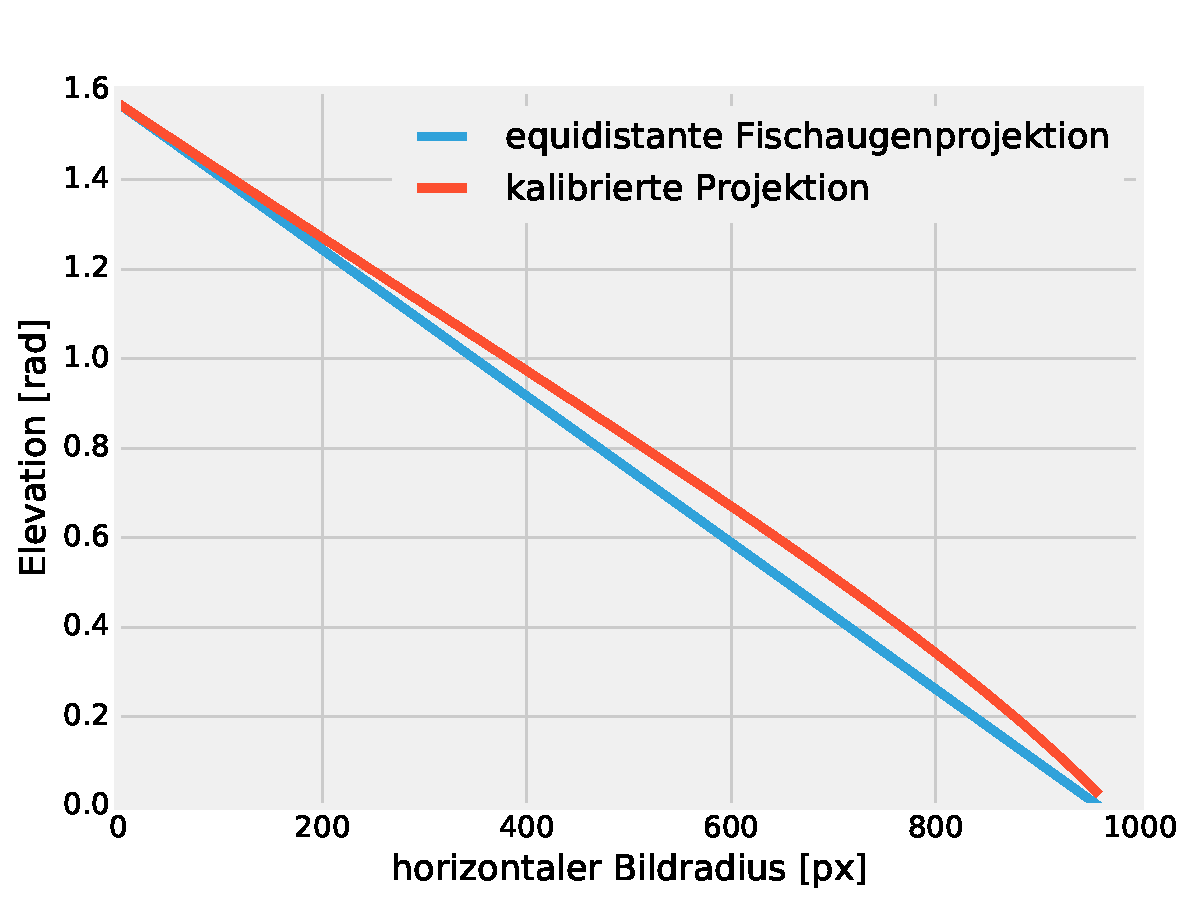
\includegraphics[width=0.5\textwidth]{media/projection-calibration.pdf}
\vspace{-0.7cm}
\caption[kalibrierte Projektionsfunktion]{kalibriertes Projektionspolynom im
Vergleich zur equidistanten Fischaugenprojektion}
\label{FIGProjektioncalib}
\end{center}
\end{figure}


%\newpage

%%%%%%%%%%%%%%%%%%%%%%%
%%% Wolkenerkennung %%%
%%%%%%%%%%%%%%%%%%%%%%%
\section{Wolkenerkennung}

Wolkenerkennung.
Oder in Englisch: Mett-Sching!
Machste halt k-Means...
\blindtext

%%%%%%%%%%%%%%%%%%%%%%%%
%%% Wolkenklustering %%%
%%%%%%%%%%%%%%%%%%%%%%%%
\subsection{Wolkenklusterung}

\blindtext[3]



%%%%%%%%%%%%%%%%%%%%%%
%%% Wolkenmatching %%%
%%%%%%%%%%%%%%%%%%%%%%
\subsection{Wolkenwiedererkennung}

Wolkenwiedererkennung.
\blindtext[3]


%\newpage


%%%%%%%%%%%%%%%%%%%%%%%
%%% Höhenbestimmung %%%
%%%%%%%%%%%%%%%%%%%%%%%
\section{Wolkenpositionierung}

Doppelanschnitt.
\blindtext[2]

%\newpage

%%%%%%%%%%%%%%%%%%%
%%% Validierung %%%
%%%%%%%%%%%%%%%%%%%
\section{Validierung}

Drachen und Ceilometer.
\blindtext[3]


%\newpage


%%%%%%%%%%%%%
%%% Fazit %%%
%%%%%%%%%%%%%
\section{Fazit}

Zusammenfassung.
\blindtext[3]

%\newpage % Neue Seite

%%%%%%%%%%%%%%%%%%%%%%%%%%%%
%%% Literaturverzeichnis %%%
%%%%%%%%%%%%%%%%%%%%%%%%%%%%
\literaturverzeichnis{bibliography.bib} % 



\end{document}
